% % % % % % % % % % % % % % % % % % % % % % % % % % % % % % % % % % % % % % % % % % % %
%                                                                                     %
% Short Sectioned Assignment LaTeX Template Version 1.0 (5/5/12)                      %
% This template has been downloaded from: http://www.LaTeXTemplates.com               %
%                                                                                     %
% Original author:  Frits Wenneker (http://www.howtotex.com)                          %
%                                                                                     %
% Modified by: Fco Javier Sueza Rodríguez (fcosueza@disroot.org)                      %
%                                                                                     %
% Changes:                                                                            %
%	    - Custom Chapters, Sections and Subsections (titlesec package)                %
%           - Document type scrbook (oneside)                                         %
%           - Use babel-lang-spanish package and marvosym                             %
%           - Use hyperref, enumitem, tcolorbox and glossaries packages               %
%           - Use Time New Roman (mathptmx), Helvetic and Courier fonts               %
%                                                                                     %
% License: CC BY-NC-SA 3.0 (http://creativecommons.org/licenses/by-nc-sa/3.0/)        %
%                                                                                     %
% % % % % % % % % % % % % % % % % % % % % % % % % % % % % % % % % % % % % % % % % % % %

%-----------------------------------------------%
%	              Packages                  %
%-----------------------------------------------%

\documentclass[paper=a4, fontsize=11pt, oneside]{scrbook}

% ---- Text Input/Output ----- %

\usepackage[T1]{fontenc}
\usepackage[utf8]{inputenc}
\usepackage{mathptmx}
\usepackage[scaled=.92]{helvet}
\usepackage{courier}
\usepackage[indent=12pt]{parskip}

\usepackage{geometry}
\geometry{verbose,tmargin=3cm,bmargin=3cm,lmargin=2.6cm,rmargin=2.6cm}

% ---- Language ----- %

\usepackage[spanish]{babel}
\usepackage{marvosym}

% ---- Another packages ---- %

\usepackage{amsmath,amsfonts,amsthm}
\usepackage{graphics,graphicx}
\usepackage{titlesec}
\usepackage{fancyhdr}
\usepackage{tcolorbox}
\usepackage{hyperref}
\usepackage{enumitem}
\usepackage[automake]{glossaries}

%--------------------------------------------------------------------%
%                      Customizing Document                          %
%--------------------------------------------------------------------%


% ----------- Custom Chapters, Sections and Subsections -------------- %

\titleformat{\chapter}[display]
			{\bfseries\Huge}
			{Tema \ \thechapter} {0.5ex}
			{\vspace{1ex}\centering}

\titleformat{\section}[hang]
			{\bfseries\Large}
			{\thesection}{0.5em}{}

\titleformat{\subsection}[hang]
			{\bfseries\large}
			{\thesubsection}{0.5em}{}

\titleformat{\subsubsection}[hang]
			{\bfseries\large}
			{\thesubsubsection}{0.5em}{}

\hypersetup{
    colorlinks=true,
    linkcolor=black,
    urlcolor=magenta
}

% ------------------- Custom heaaders and footers ------------------- %

\pagestyle{fancyplain}

\fancyhead[]{}
\fancyfoot[L]{}
\fancyfoot[C]{}
\fancyfoot[R]{\thepage}

\renewcommand{\headrulewidth}{0pt} % Remove header underlines
\renewcommand{\footrulewidth}{0pt} % Remove footer underlines

\setlength{\headheight}{13.6pt} % Customize the height of the header

% --------- Numbering equations, figures and tables ----------------- %

\numberwithin{equation}{section} % Number equations within sections
\numberwithin{figure}{section} % Number figures within sections
\numberwithin{table}{section} % Number tables within sections

% ------------------------ New Commands ----------------------------- %

\newcommand{\horrule}[1]{\rule{\linewidth}{#1}} % Create horizontal rule command


%----------------------------------------------------------------------------------------
%	TÍTULO Y DATOS DEL ALUMNO
%----------------------------------------------------------------------------------------

\title{
\vspace{10ex}
\normalfont \normalsize
\huge \textbf{Documentación Tarea 6}
}
\author{Francisco Javier Sueza Rodríguez}
\date{\normalsize\today}

%----------------------------------------------------------------------------------------
%                                     DOCUMENTO
%----------------------------------------------------------------------------------------
\begin{document}

\maketitle

\thispagestyle{empty}

\vspace{75ex}

\begin{center}
    \begin{tabular}{l l}
        \textbf{Centro}: & IES Aguadulce \\
        \textbf{Ciclo Formativo}: & Desarrollo Aplicaciones Web (Distancia)\\
        \textbf{Asignatura}: & Diseño de Interfaces Web\\
        \textbf{Tema}: & Tema 6 -  Contenidos Web Interactivos\\
    \end{tabular}
\end{center}

\newpage

\section{Introducción}
En este documento se van a especificar diferentes aspecto de la web desarrollada para la tarea 6 de la asignatura Desarrollo de Interfaces Web.

Se han realizado pruebas en diferentes navegadores, siendo los escogidos Chrome y Mozilla Firefox, de las cuales se incluyen varias capturas, además se especificará los filtros que se han seleccionado para aplicar al collage, así como las fuentes elegidas para el cambio de letra en la sección de texto.

Además, se incluirán las fuentes y autoría de las imágenes empleadas en la web, así como una última sección TODO donde se incluirá que falta por hacer en la web.


\section{Estructura del Proyecto}
El proyecto se ha estructurado siguiente un patrón modular. En el archivo \textbf{index.html} se ha cargado solo el archivo JS princial \textbf{main.js}, que es el encargado de añadir los gestores de eventos a todos los elementos de la página importando para ello los diferentes archivos que contiene las funciones para cada una de las secciones.

Además de estos archivos, se ha incluido el archivo \textbf{default.js} donde se definen todas las contantes para especificar el estado inicial de la aplicación, de esta forma, podemos cambiar el estado inicial de ésta de forma rápida y sencilla.

Además se ha documentado todo el código empleando la sintaxis \textbf{JSDoc}, de forma que si quisiéramos generar la documentación del proyecto simplemente deberíamos instalar el paquete adecuado y ejecutarlo.

\section{Fuentes y Filtros Seleccionados}
Para la \textbf{sección de imágenes}, se han seleccionado diferentes filtros aplicados con un porcentaje predefinido, estos \textbf{filtros} han sido los siguientes:

\begin{itemize}
    \item \textbf{contrast}: filtro que cambia el contraste de la imagen, aplicado en un \textbf{200\%} para que el cambio sea apreciable.
    \item \textbf{saturation}: filtro que cambia la saturación de la imagen, aplicado en un \textbf{150\%}.
    \item \textbf{grayscale}: filtro que cambia el color de la imagen a una escala de grises, aplicado en un \textbf{100\%}.
    \item \textbf{invert}: filtro que invierte los colores de imagen creando una imagen en negativo, aplicado en un \textbf{100\%}.
\end{itemize}

Además de estos filtros, se ha proporcionado la opción \textbf{Ninguno}, que establece la opción CSS \textbf{filter} a \textbf{none} y
elimina cualquier filtro que estuviera aplicado a la imagen que pulsemos.

Por otro lado \textbf{las fuentes} seleccionadas han sido fuentes seguras para que se puedan ejecutar en cualquier navegador, sin que podamos tener algún problema ni la necesidad de instalar ninguna fuente de forma local o importarla. Así, las fuentes seleccionadas han sido:

\begin{itemize}
    \item Arial
    \item Times New Roman
    \item Cursive
    \item Monospace
\end{itemize}

Estás fuentes no deben generar ningún problema en su visualización en cualquier navegador.

\section{Autoría y Licencia de las Imágenes Empleadas}
Las imágenes empleadas han sido generadas en la plataforma \href{https://deepai.org/}{DeepAI}. La licencia empleada se especifica en los \href{https://deepai.org/terms-of-service/terms-of-service}{terminos de uso} que se especifica en la página web, en concreto en el apartado \textbf{General Content License}, que rige el contenido generado con la aplicación.

Según esta licencia, se garantiza el uso de de las imágenes generadas para cualquier propósito, ya sea este comercial o no, siempre y cuando no entrañe una actividad ilegal.

Respecto a la \textbf{autoría}, la imágenes han sido generadas por la plataforma siguiendo mis especificaciones y configuración.

\section{Pruebas en Navegadores}
Para la realización de la pruebas, se han utilizado los navegadores \textbf{Chrome} en su versión \textbf{124.0.63} y \textbf{Mozilla Firefox Developer Edition}, en su versión \textbf{127.0b1}. Se han seleccionado estos dos navegadores porque además de ser los más usados, ambos tienen \textbf{motores de renderizado diferentes}, en concreto, el motor de Chrome es \textbf{Blink} mientras que el motor de Firefox es \textbf{Gecko}.

En \textbf{primer lugar} se ha testeado en \textbf{Mozilla Firefox}, para ello se han aplicado diferente filtros a las imágenes del collage, además de cambiar el color del borde, su grosor y la disposición del collage a vertical. Además, se ha cambiado la fuente de la letra del texto, así como su espaciado, pulsando a continuación del botón para mostrar el segundo título, como podemos ver en la siguiente captura.

\begin{figure}[H]
    \centering
    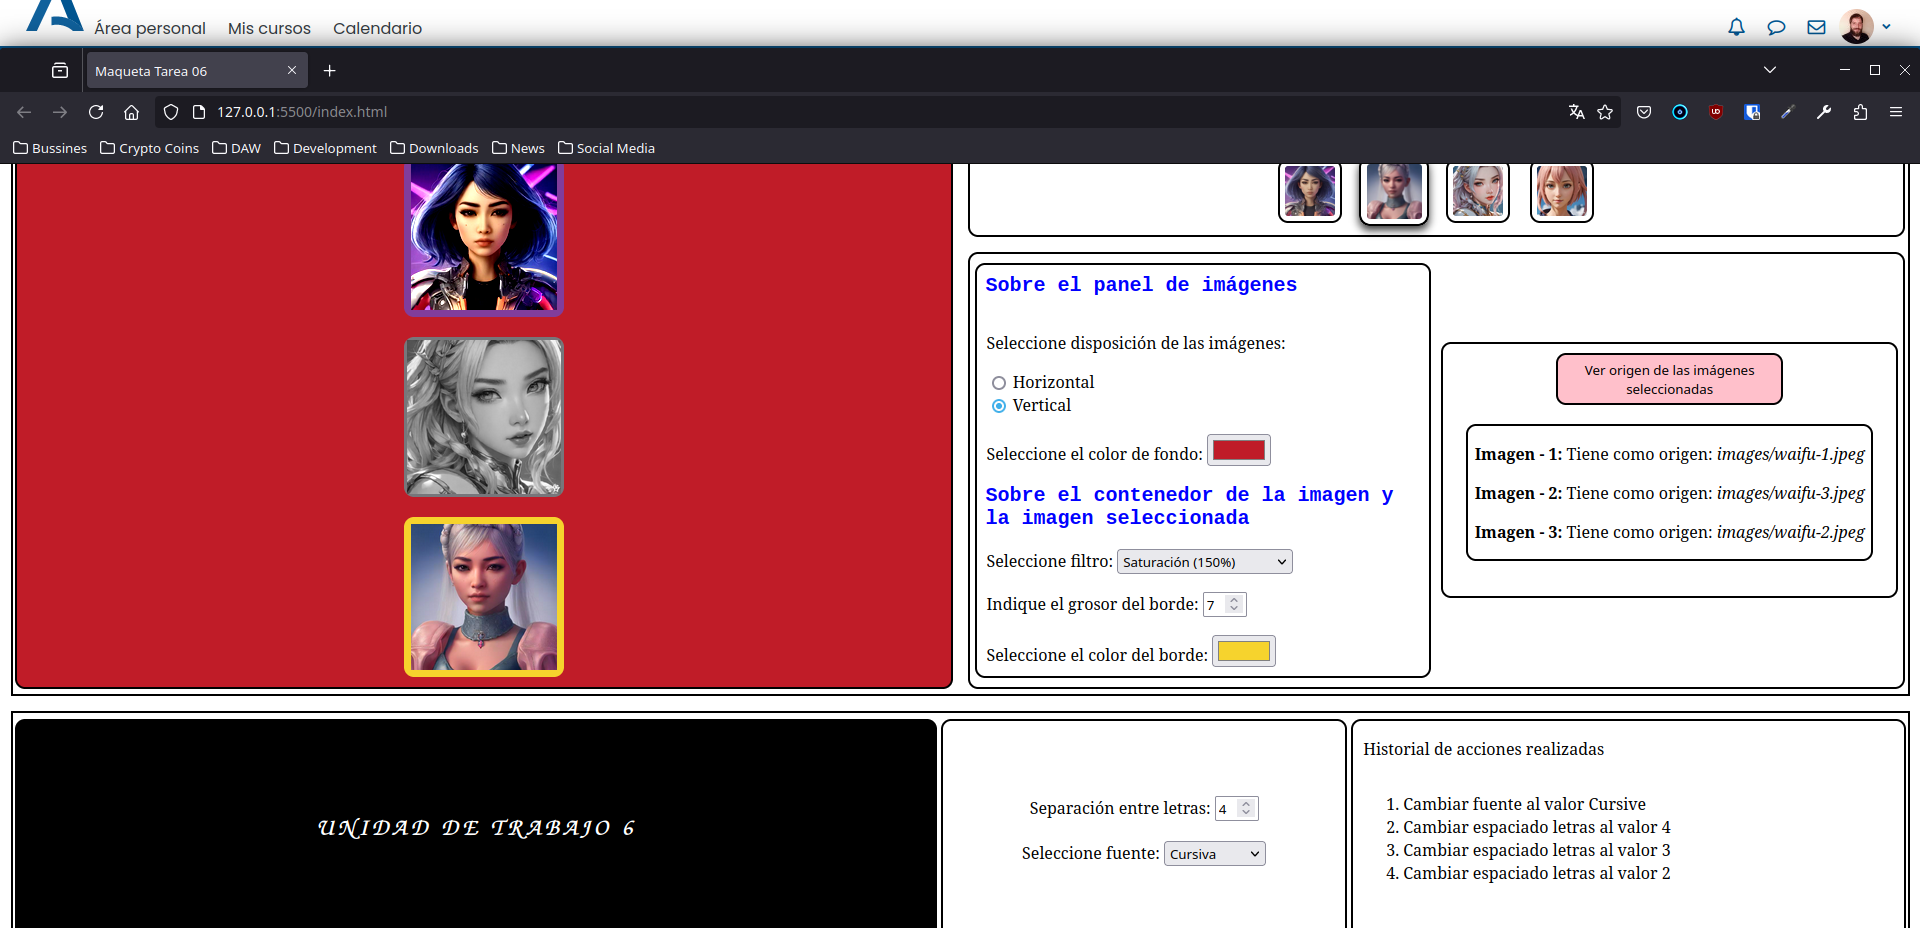
\includegraphics[scale=0.25]{mozilla-1.png}
    \caption{Visualización de la página en Mozilla Firefox}
\end{figure}

Como podemos ver, todos los efectos se han aplicado correctamente, así como se ha actualizado el historial de acciones y se ha mostrado correctamente las fuentes de las imágenes cargadas en el collage.

Lo siguiente que se ha realizado ha sido una \textbf{inicialización} de la web, empleando para ello el botón de inicializar para comprobar que la web vuelve a su estado inicial, así como que el historial de la aplicación se mantiene, como podemos ver en al siguiente captura.

\begin{figure}[H]
    \centering
    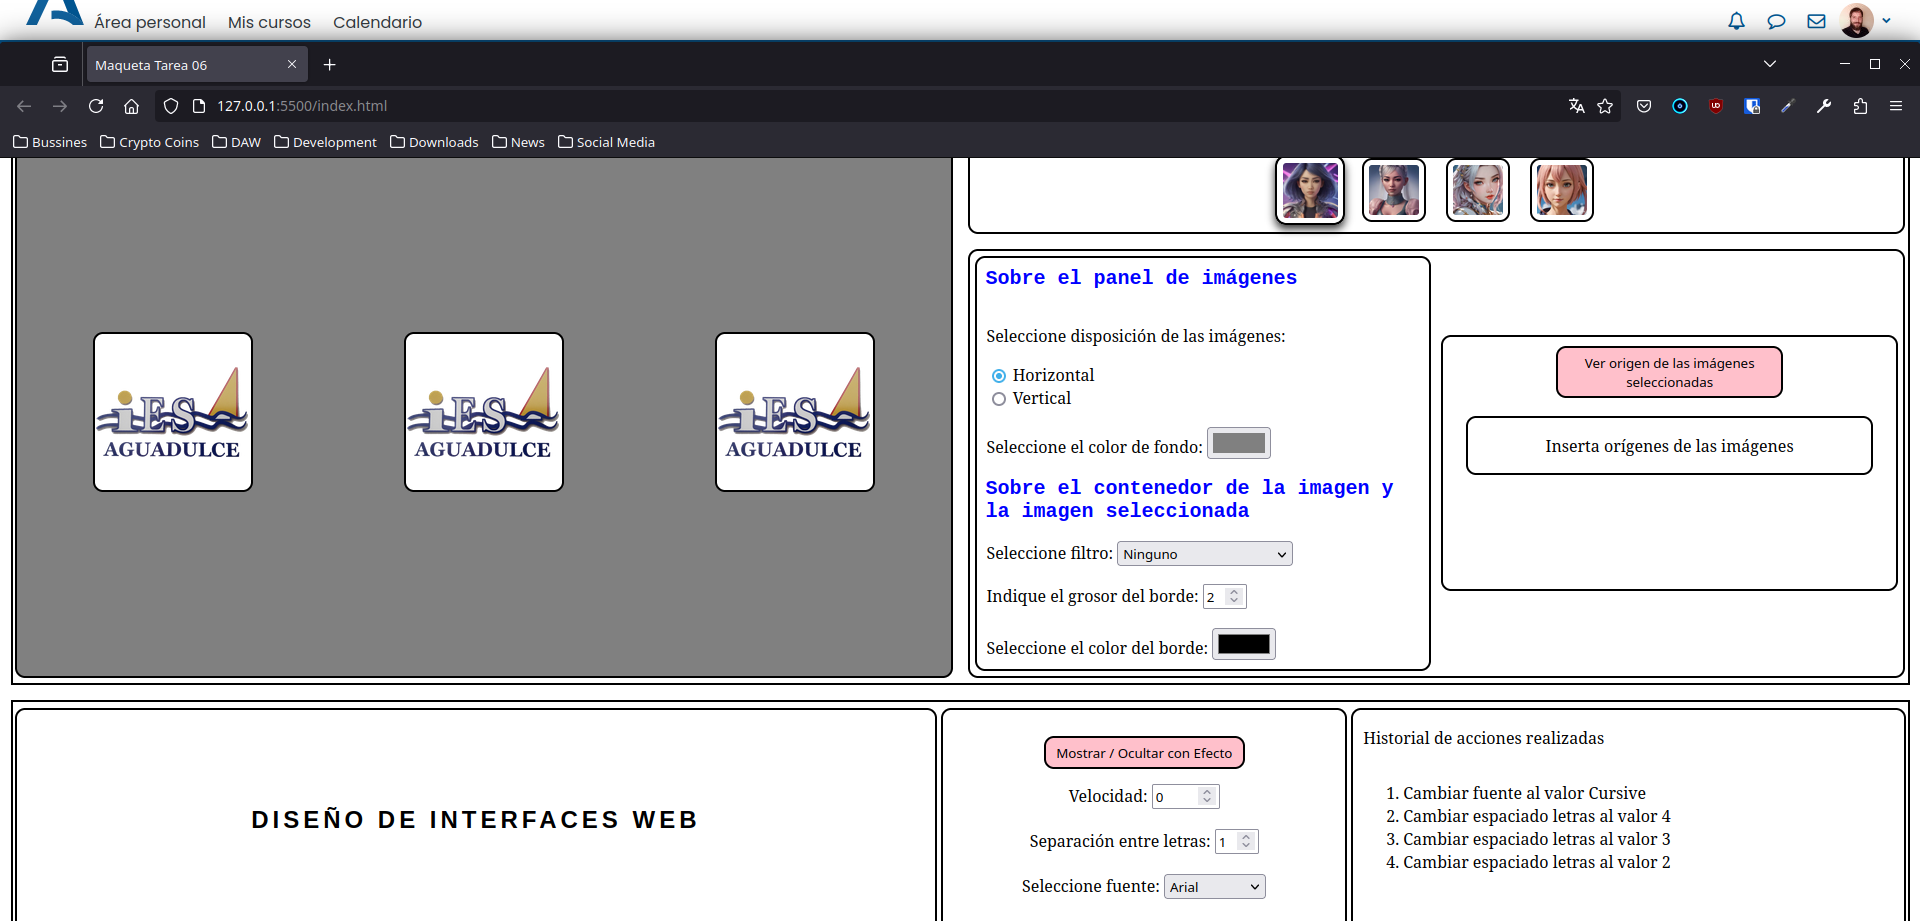
\includegraphics[scale=0.25]{mozilla-2.png}
    \caption{Inicializado de la página usando el botón Inicializar}
\end{figure}

A continuación se han realizado las mismas acciones, que no vamos a duplicar su explicación, en Chrome, pudiendo ver los resultados en las siguiente 2 capturas.

\begin{figure}[H]
    \centering
    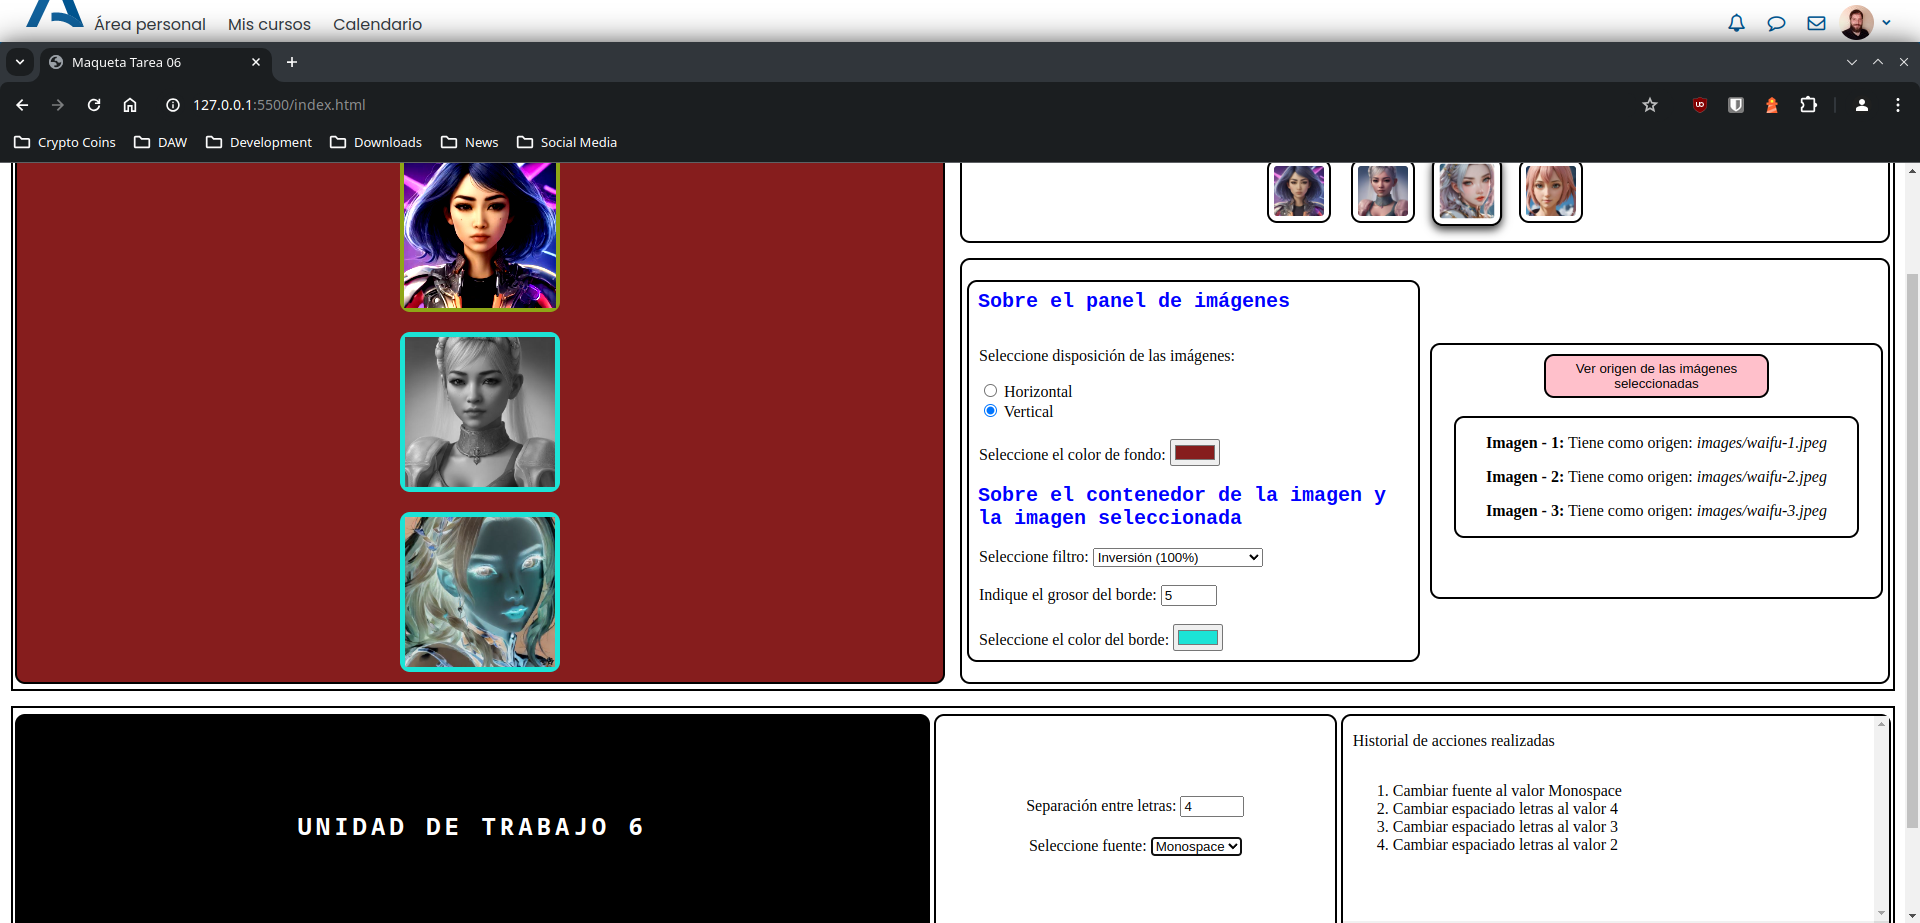
\includegraphics[scale=0.24]{chrome-1.png}
    \caption{Visualizaciónd de la página web en Google Chrome}
\end{figure}

\begin{figure}[H]
    \centering
    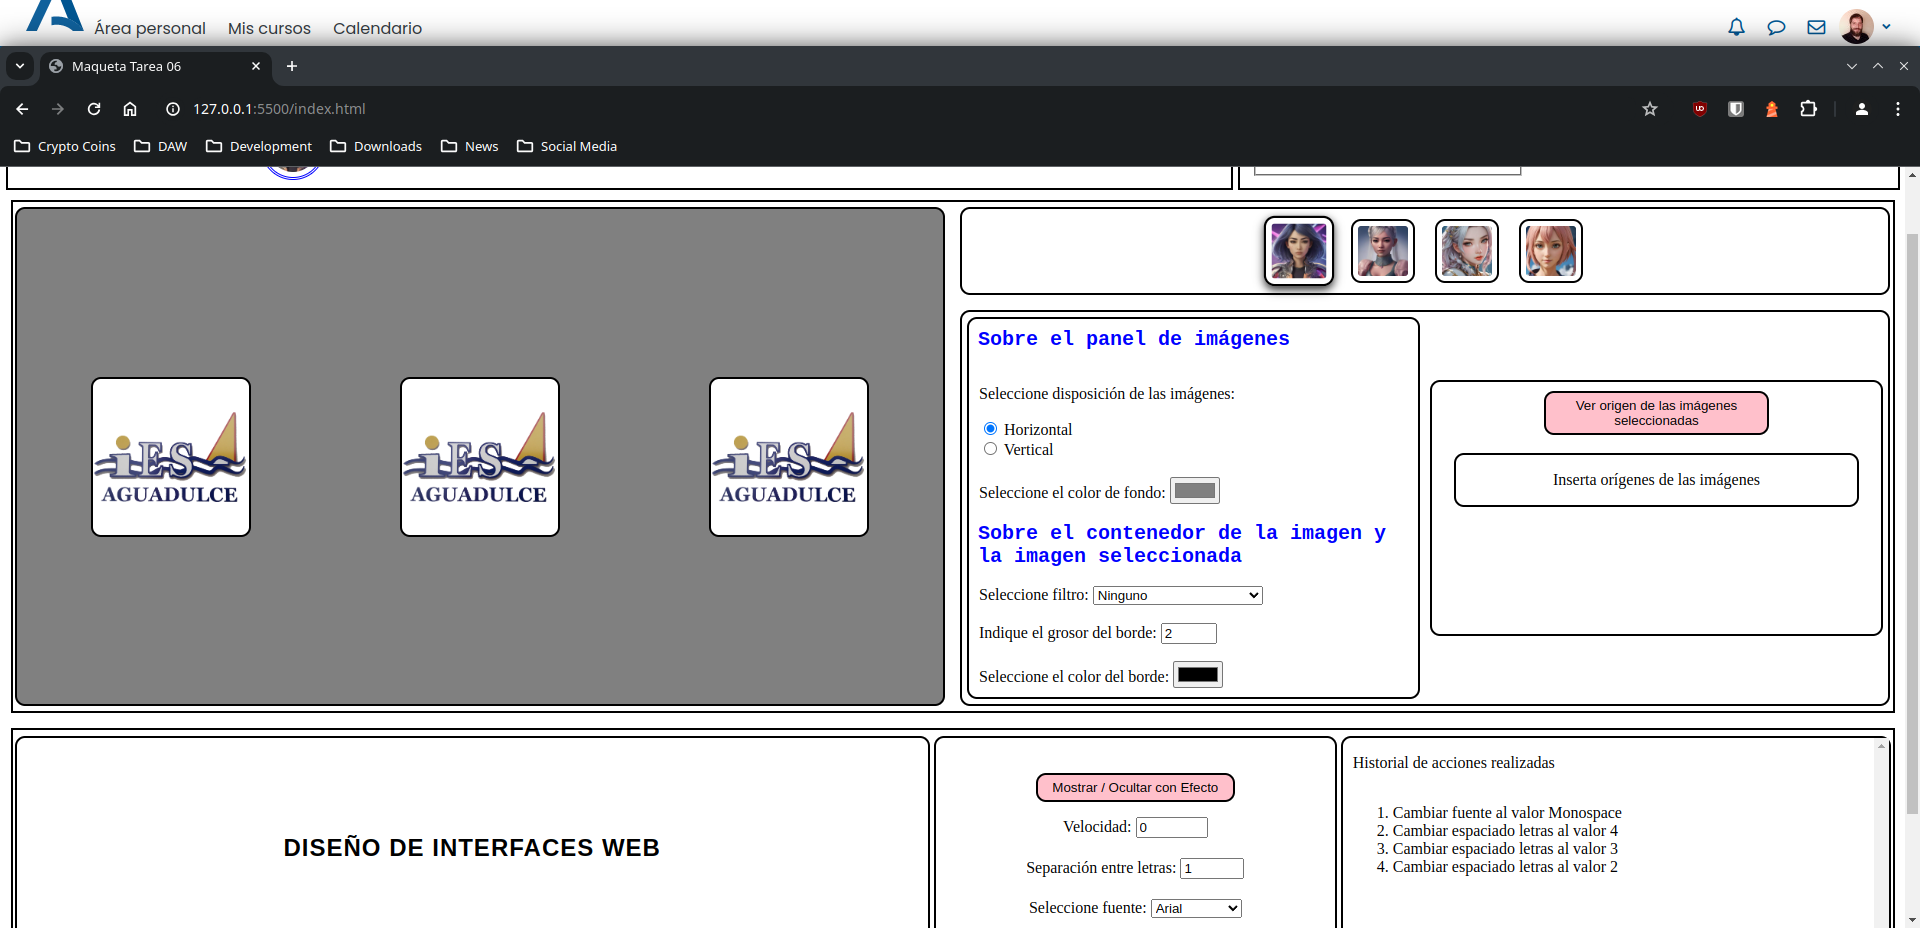
\includegraphics[scale=0.24]{chrome-2.png}
    \caption{Inicializado de la página usando el botón Inicializar en Chrome}
\end{figure}

Como podemos ver en las capturas aportadas, la aplicación de los efectos así como el reinicio de la página a su estado inicial se lleva a cabo correctamente tanto en Google Chrome como en Mozilla Firefox.


% Bibliography

%\newpage
%\bibliography{citas}
%\bibliographystyle{unsrt}

\end{document}